% !TEX root = ../main.tex
% Chapter 5

\chapter{Artificial data results}

\label{Chapter5} % For referencing the chapter elsewhere, use~\ref{Chapter5}

\lhead{Chapter 5. \emph{Artificial data results}} % This is for the header on each page - perhaps a shortened title

%----------------------------------------------------------------------------------------
\section{Outline}
\emph{Not intented for the reader.}
\begin{itemize}
  \item Compare proposed method with methods of \Cref{Chapter2}
  \item Provide KL-analysis (as Takeuchi does)
  \item Provide plots, tables, graphs, error rates, precision, etc.
  \item Apply to a multiple of data, to compare to previous research - use that data
  \item Give theoretical analysis about performance. Big-O, memory, run-time, precision.
  \item This sections needs programmed implementations of own method and the ones compared
\end{itemize}

In this chapter we will apply the proposed algorithm to artificial data sets.
For comparison, we use some of the data sets that are used by Camci~\cite{camci2010change} and Takeuchi \etal \cite{takeuchi2006unifying}.
These data sets are generated by Gaussian noise distributions.
In \Cref{sec:artificial_data_generation} the precise generation method and characteristics of the data sets are discussed.
For our final change detection mechanism we use the \gls{rt}-method, also applied by Camci \cite{camci2010change}.
This is a simple and fast method and allows us to mainly focus on the \gls{oc-svm} model properties that should reflect changes in the data.
The results of these two methods are discussed in \Cref{sec:artificial_data_results}.

% !TEX root = ../../main.tex
\section{Artifical data generation}\label{sec:artificial_data_generation}
\TODO{Use data from \cite{camci2010change,takeuchi2006unifying}}
In this section we present three data sets as used by \cite{camci2010change,takeuchi2006unifying} to provide for a objetive performance comparison.

Model:
\begin{equation}
  x_t = a_1 x_{t-1} + a_2 x_{t-2} + \epsilon_t,
\end{equation}
where $\epsilon_t$ is a Gaussian distribution, modeling the noise.
The length of $x_t$ is $10000$ and change points are generated at each $y \times 10000^\text{th}$ data point, with $y = (1, 2, 3, \dots 9)$.

\begin{figure}
\centering
  \includegraphics[width=1\textwidth]{./Figures/notes/jumping_mean_takeuchi.eps}
  \caption[Jumping mean Takeuchi, set 1]{Jumping mean takeuchi, set 1}
  \label{fig:jumping_mean_takeuchi}
\end{figure}

\begin{figure}
\centering
  \includegraphics[width=1\textwidth]{./Figures/notes/jumping_mean_takeuchi_thresholds.eps}
  \caption[Jumping mean Takeuchi, set 1, thresholds]{Jumping mean takeuchi, set 1, thresholds}
\end{figure}


First Takeuchi, reduced jumping mean, Figure~\ref{fig:jumping_mean_takeuchi}:
$\epsilon_t$ is Gaussian with mean $0$ and variance $\sigma^2 = 1$, $a_1 = 0.6$ and $a_2 = -0.5$.

\begin{figure}
\centering
  \includegraphics[width=1\textwidth]{./Figures/notes/jumping_variance_mean_takeuchi.eps}
  \caption[Jumping variance and mean Takeuchi, set 2]{Jumping variance and mean takeuchi, set 2}
  \label{fig:jumping_variance_and_mean_takeuchi}
\end{figure}

\begin{figure}
\centering
  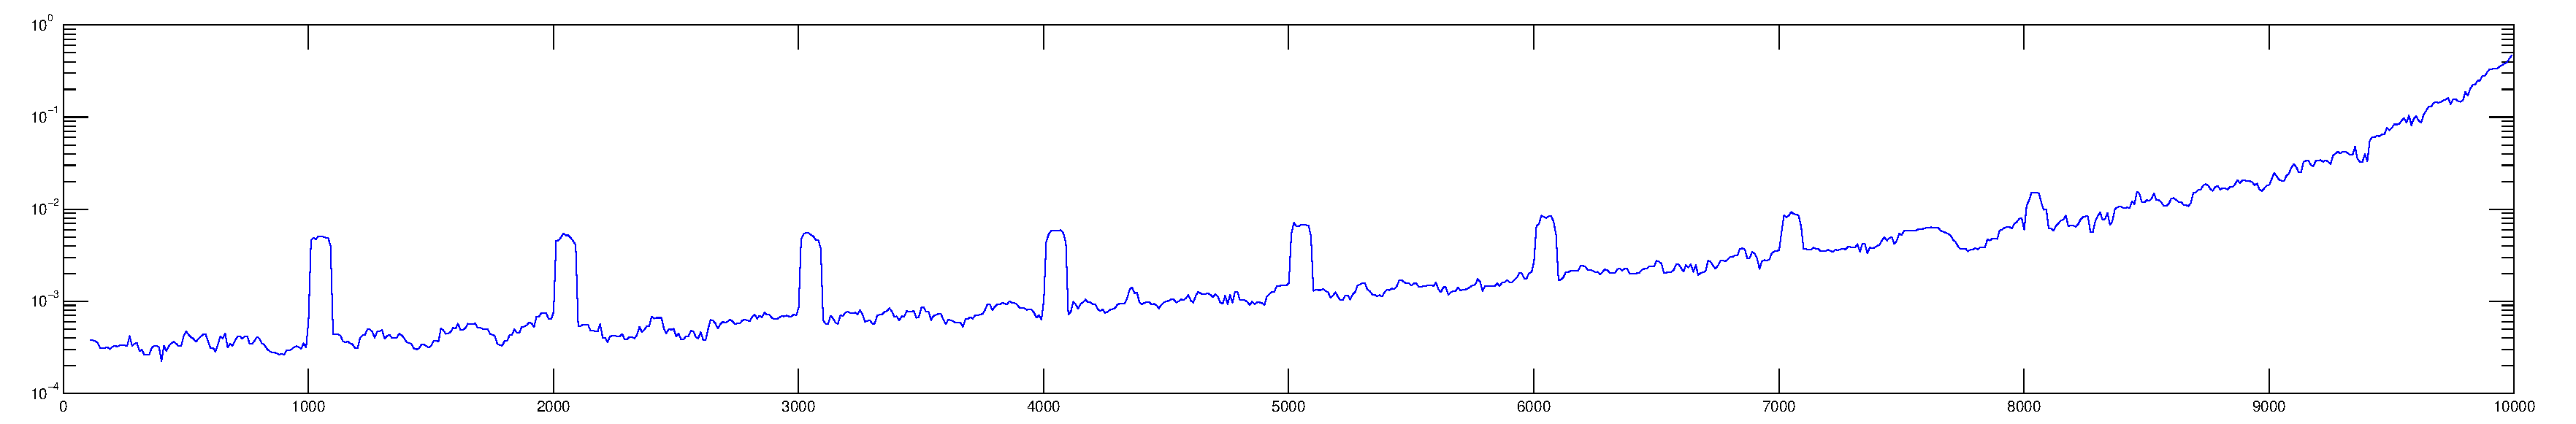
\includegraphics[width=1\textwidth]{./Figures/notes/jumping_variance_mean_takeuchi_thresholds_log_scale.eps}
  \caption[Jumping variance mean Takeuchi, set 2, thresholds]{Jumping variance and mean takeuchi, set 2, thresholds (log scale)}
\end{figure}

Second Takeuchi, jumping mean with $\Delta y = 1$ and $\sigma^2 = 0.1 / (0.01 + (10000 - x)/1000)$.
Figure~\ref{fig:jumping_variance_and_mean_takeuchi}.

\begin{figure}
\centering
  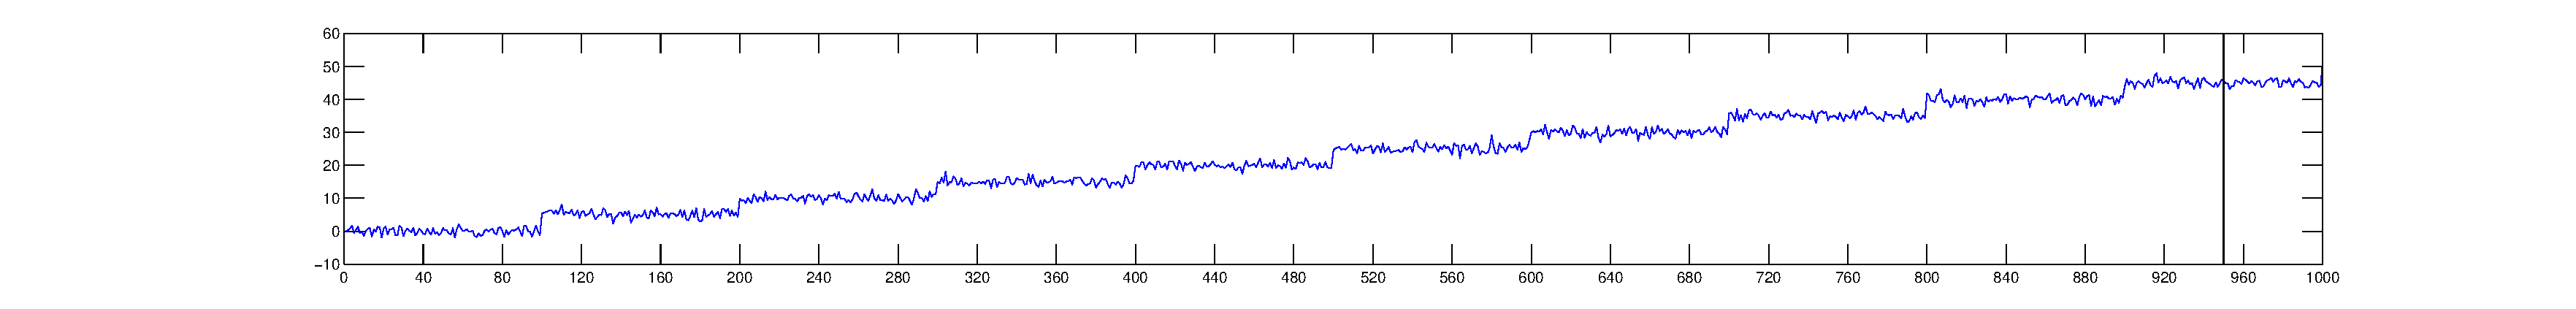
\includegraphics[width=1\textwidth]{./Figures/notes/jumping_mean_camci.eps}
  \caption[Jumping mean camci]{Jumping mean camci}
  \label{fig:camci_mean_fixed}
\end{figure}

First Camci, fixed jumping mean.
$\Delta y = 5$
See Figure~\ref{fig:camci_mean_fixed}.


\begin{figure}
\centering
  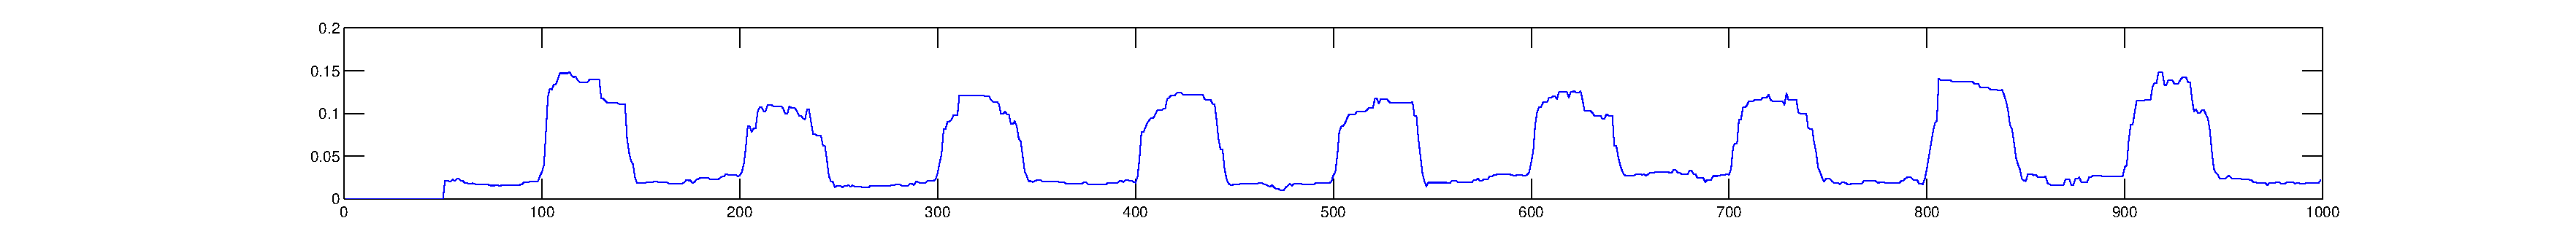
\includegraphics[width=1\textwidth]{./Figures/notes/jumping_mean_camci_thresholds.eps}
  \caption[Jumping mean camci thresholds]{Jumping mean camci, thresholds}
\end{figure}

\begin{figure}
\centering
  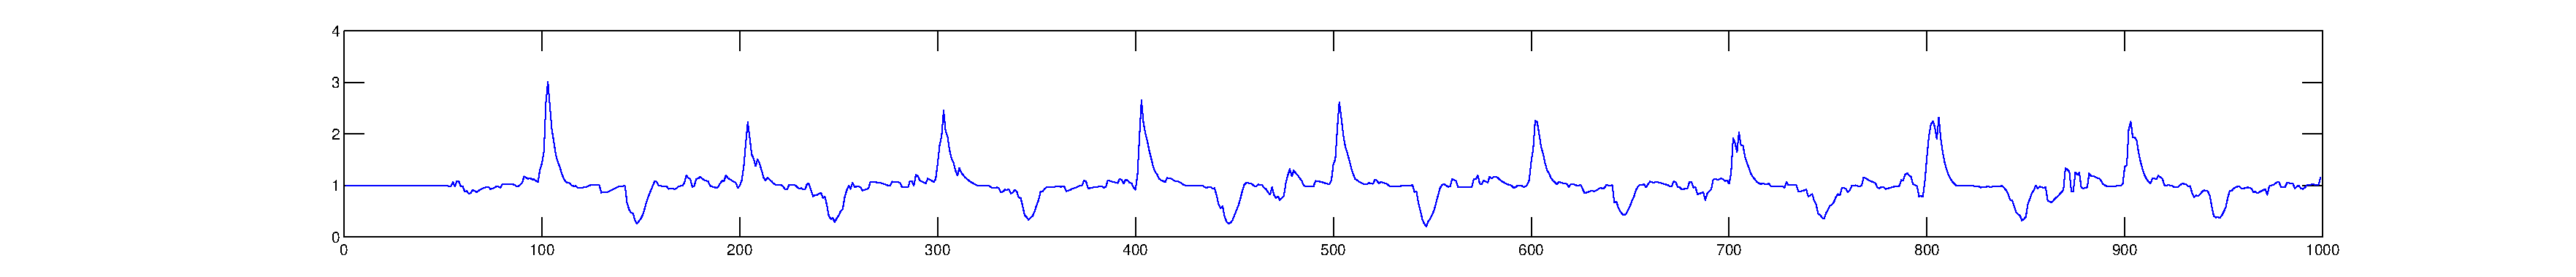
\includegraphics[width=1\textwidth]{./Figures/notes/jumping_mean_camci_ratios_10.eps}
  \caption[Jumping mean camci ratios]{Jumping mean camci ratios, last 10}
  \label{fig:jumping_mean_ratios}
\end{figure}

\begin{figure}
\centering
  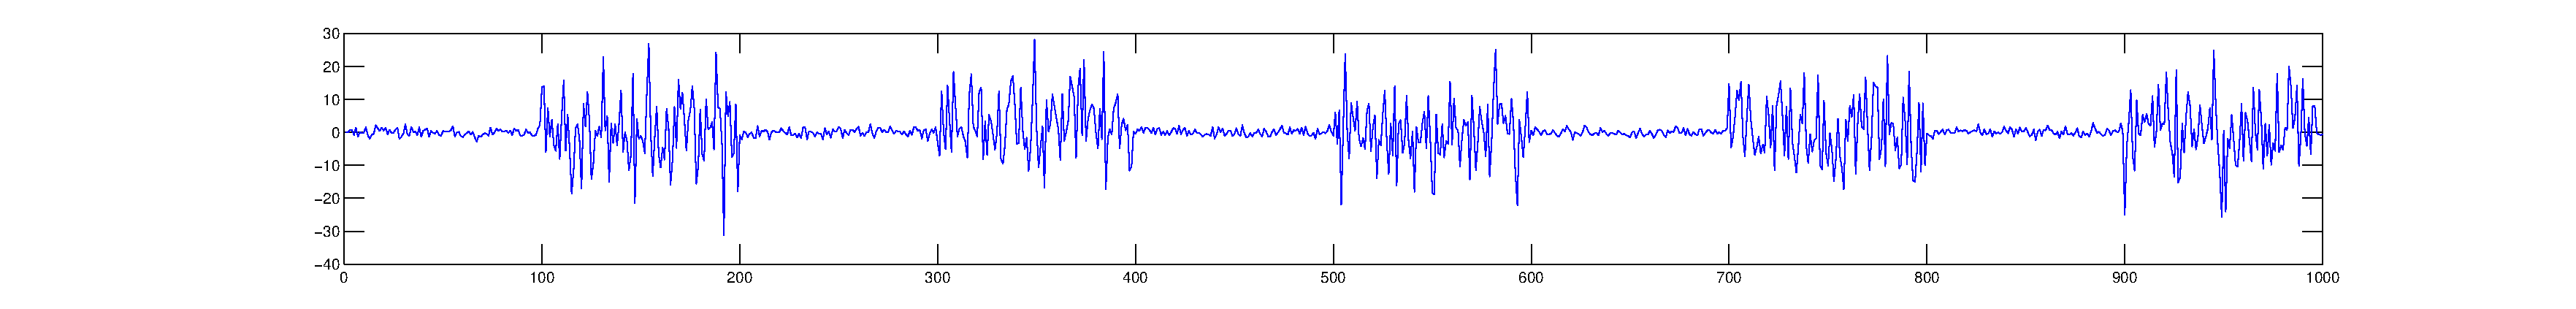
\includegraphics[width=1\textwidth]{./Figures/notes/jumping_variance.eps}
  \caption[Jumping variance]{Jumping variance, equal for Camci and Takeuchi, both set 3}
  \label{fig:jumping_variance_camci_takeuchi}
\end{figure}

Third Camci and Takeuchi, jumping variance.
When $y$ is odd, variance $\sigma^2$ changes from $1.0$ to $9.0$, and when $y$ is even variance $\sigma^2$ changes from $9.0$ to $1.0$.
See Figure~\ref{fig:jumping_variance_camci_takeuchi}.

\begin{figure}
\centering
  \includegraphics[width=1\textwidth]{./Figures/notes/jumping_variance_thresholds.eps}
  \caption[Jumping variance thresholds]{Jumping variance, thresholds}
\end{figure}

\begin{figure}
\centering
  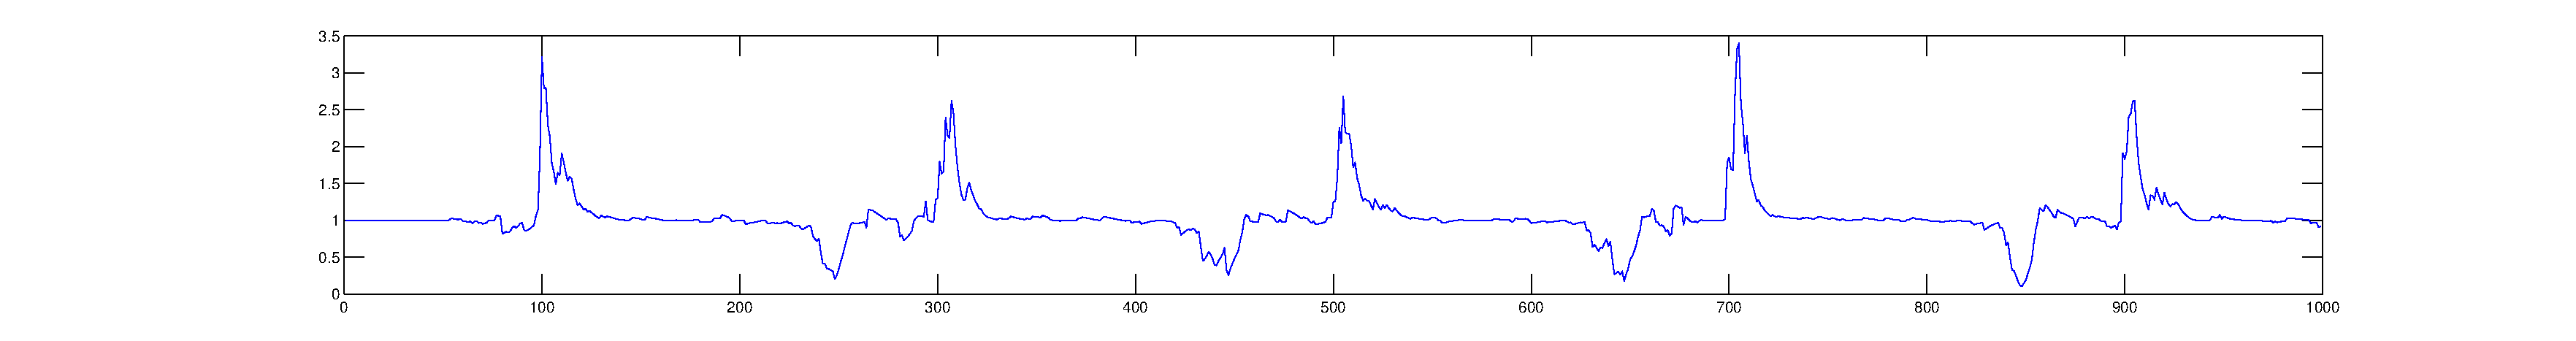
\includegraphics[width=1\textwidth]{./Figures/notes/jumping_variance_ratios_10.eps}
  \caption[Jumping variance ratios]{Jumping variance ratios, last 10}
\end{figure}


% !TEX root = ../../main.tex
\section{Results}\label{sec:artificial_data_results}
The results of all the data sets are provided in \Cref{tab:results_artificial}, together with the used parameters.
For each data set it shows the high and low thresholds used in the \gls{rt} based change detection method.
During the post-processing all detected change points within a certain \emph{closeness} range are merged, for which the value differs per data set.
The difference between the actual and final detected change points are expressed as an offset.
The data sets were processed with different window lengths and $\sigma$ value for the \gls{rbf} kernel.

\begin{table}
  \centering
  \caption[Results artificial data sets]{Parameter settings and results of the artificial data sets.}
  \begin{tabulary}{\textwidth}{|l|c|c|c|c|}
    \cline{2-5}
    \multicolumn{1}{l|}{} & Set 1 & Set 2 & Set 3 & Set 4 \\
    \hline
    Window length & 50 & 100 & 50 & 50 \\
    \hline
    Sigma of \gls{rbf} & 13 & 13 & 15 & 13 \\
    \hline
    High threshold & 1.6 & 1.6 & 1.5 & 2.2 \\
    \hline
    Low threshold & 0.1 & 0.1 & 0.5 & 0.1 \\
    \hline
    Closeness & 10 & 10 & 10 & 50 \\
    \hline
    \hline
    $\gamma(Y)$ & 0 & 0.1 & 0.1 & 0.1 \\
    \hline
    $d_{avg}$ & 2.27 & 6.18 & 0.64 & 15.36 \\
    \hline
    $std(d_{avg})$ & 1.19 & 7.94 & 0.92 & 17.70 \\
    \hline
  \end{tabulary}
  \label{tab:results_artificial}
\end{table}

\begin{figure}
\centering
  \includegraphics[width=1\textwidth]{./Figures/chapter5/boxplot_results_artificial_sets.eps}
  \caption[Box plot results artificial data sets]{Box plot of the results for the artificial data sets, indicating the number of data points between the actual and closest detected change points. A lower and more compact box plot is better.}
  \label{fig:boxplot_artificial_sets}
\end{figure}

To give a better impression of the spread of the accuracy of the detected change points, a box plot for each data set is displayed in \Cref{fig:boxplot_artificial_sets} and are the results are visualized in \Cref{fig:plots_results_artificial_data_sets}.
This last figure shows the number of data points between each actual and closest detected change point.
Using the box plot notation, we can visualize not only the average but also the spread of the delay.
With each data set embodying different characteristics, different observations can be drawn from the data sets.
In the references figures, the solid blue line represent the radius of the constructed hypersphere.
The vertical dashed and thick red lines are the discovered change points.
For each data set the following is observed:
\begin{enumerate}
  \item \textbf{Fixed increasing mean:} In \Cref{fig:camci_fixed_increasing_mean_thresholds} we see that each change point is almost equally fast and accurate detected.
  This implies that the relative difference between the means of the Gaussian distribution has little effect on the detectability of the algorithm.
  \item \textbf{Reduced increasing mean:} \Cref{fig:takeuchi_reduced_increasing_mean_thresholds} shows that the absolute difference between the means of the Gaussian distribution is a certain influence to the detectability.
  Although all change points are correctly detected (at the beginning of the series are two outliers), the change in radius becomes less significant at every change point.
  \item \textbf{Reduced increasing mean, increasing variance:} In \Cref{fig:camci_takeuchi_alternating_variance_thresholds} we see the same effect, in regard to the mean, as with the previous data set.
  Furthermore, the increasing variance makes change detection harder.
  This is visible around the $9000$\textsuperscript{th} data point and after, where the radius keeps increasing.
  \item \textbf{Alternating variance:} The ability to detect decreases in variance of the Gaussian distribution is displayed in \Cref{fig:camci_reduced_increasing_mean_increasing_variance_thresholds}.
  Although some change points are discovered with a delay almost up to the length of the window processing the data, the decreases are all detected.
  The box plot of this set, number 4 in \Cref{fig:boxplot_artificial_sets}, shows a wider spread for the results.
\end{enumerate}

\begin{figure}
  \centering
  \begin{subfigure}[b]{1\textwidth}
    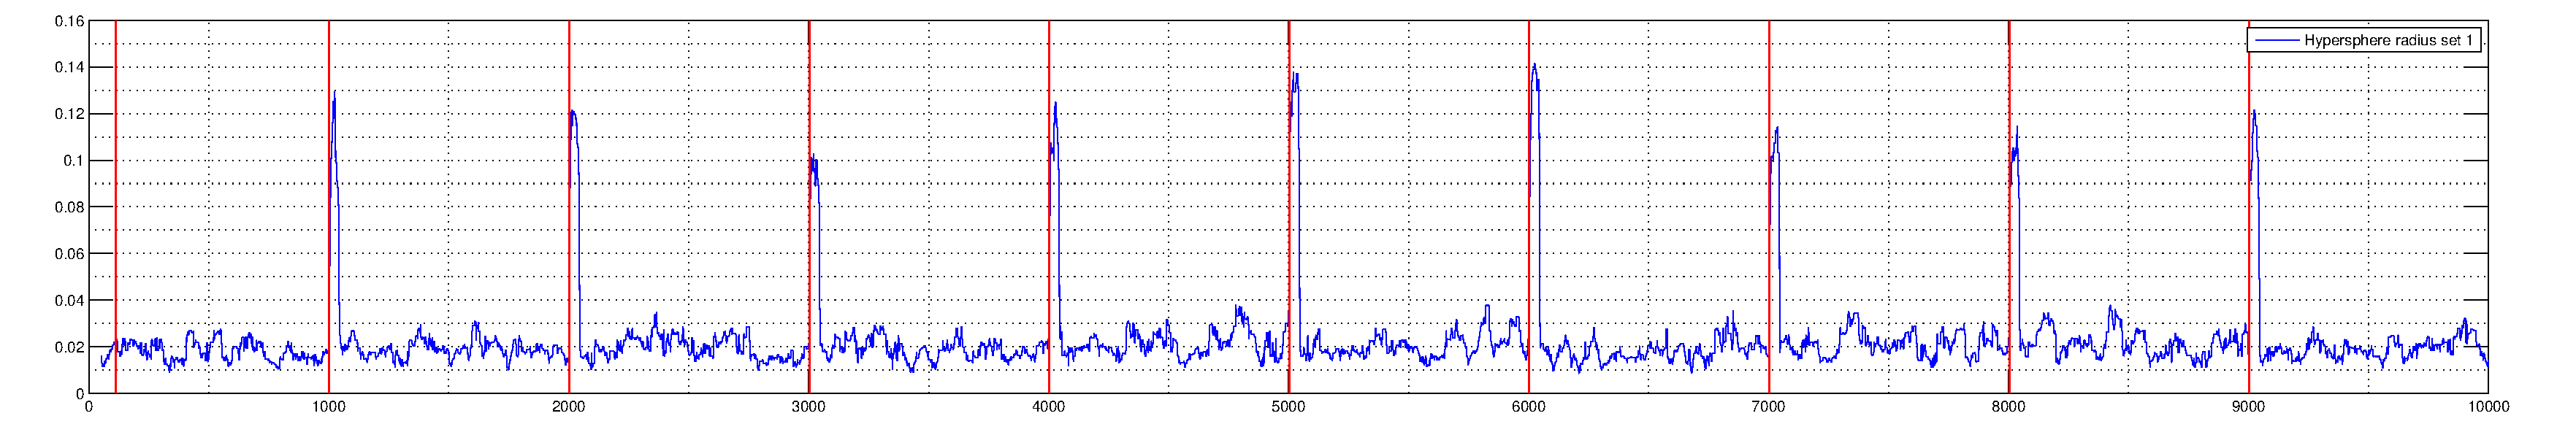
\includegraphics[width=1\textwidth]{./Figures/chapter5/set_1_results.eps}
    \caption[Fixed increasing mean, thresholds]{\emph{Fixed increasing mean} data set.}
      \label{fig:camci_fixed_increasing_mean_thresholds}
  \end{subfigure} \\

  \begin{subfigure}[b]{1\textwidth}
   \includegraphics[width=1\textwidth]{./Figures/chapter5/set_2_results.eps}
    \caption[Reduced increasing mean, thresholds]{\emph{Reduced increasing mean} data set.}
    \label{fig:takeuchi_reduced_increasing_mean_thresholds}
  \end{subfigure} \\

  \begin{subfigure}[b]{1\textwidth}
    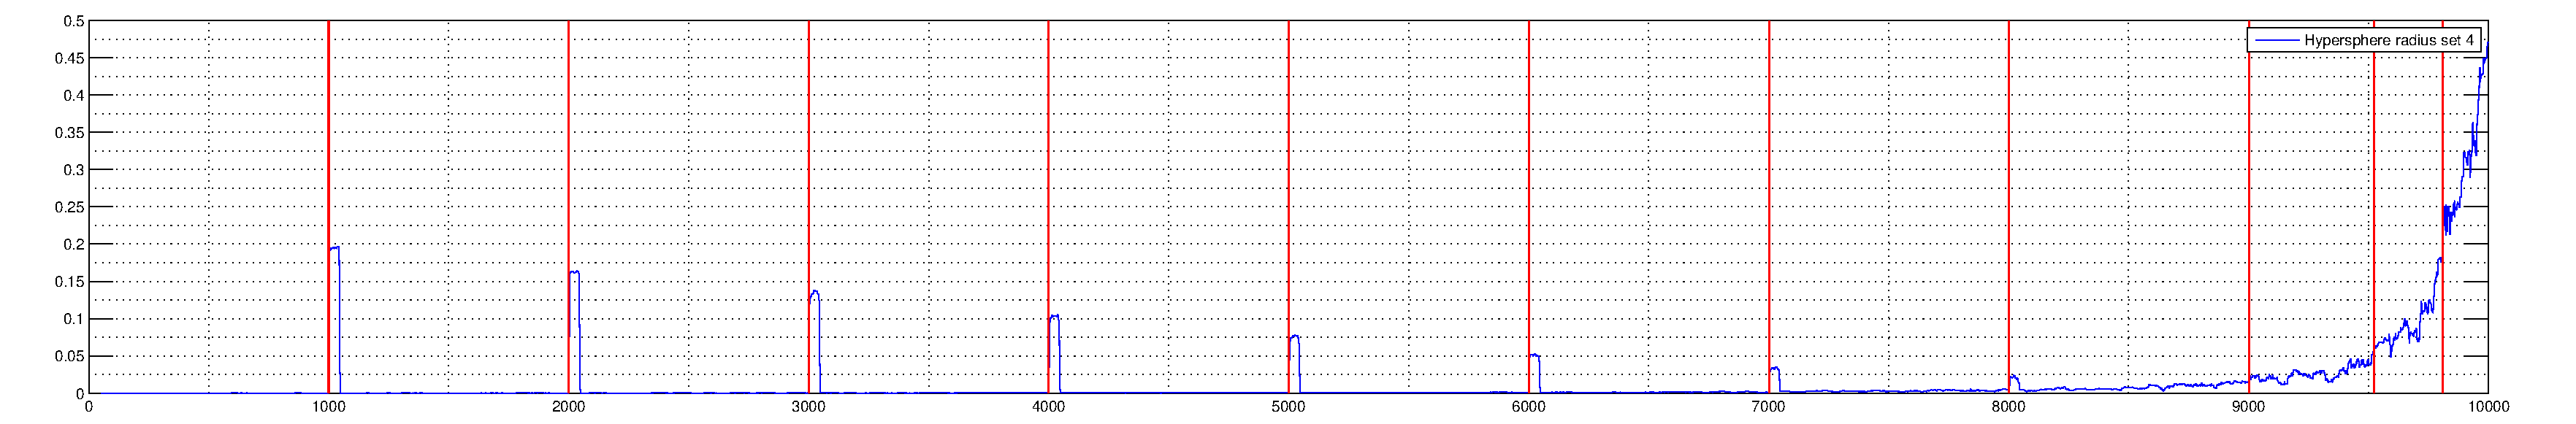
\includegraphics[width=1\textwidth]{./Figures/chapter5/set_3_results.eps}
      \caption[Reduced increasing mean, increasing variance, thresholds]{\emph{Reduced increasing mean, increasing variance} data set.}
      \label{fig:camci_reduced_increasing_mean_increasing_variance_thresholds}
  \end{subfigure} \\

  \begin{subfigure}[b]{1\textwidth}
   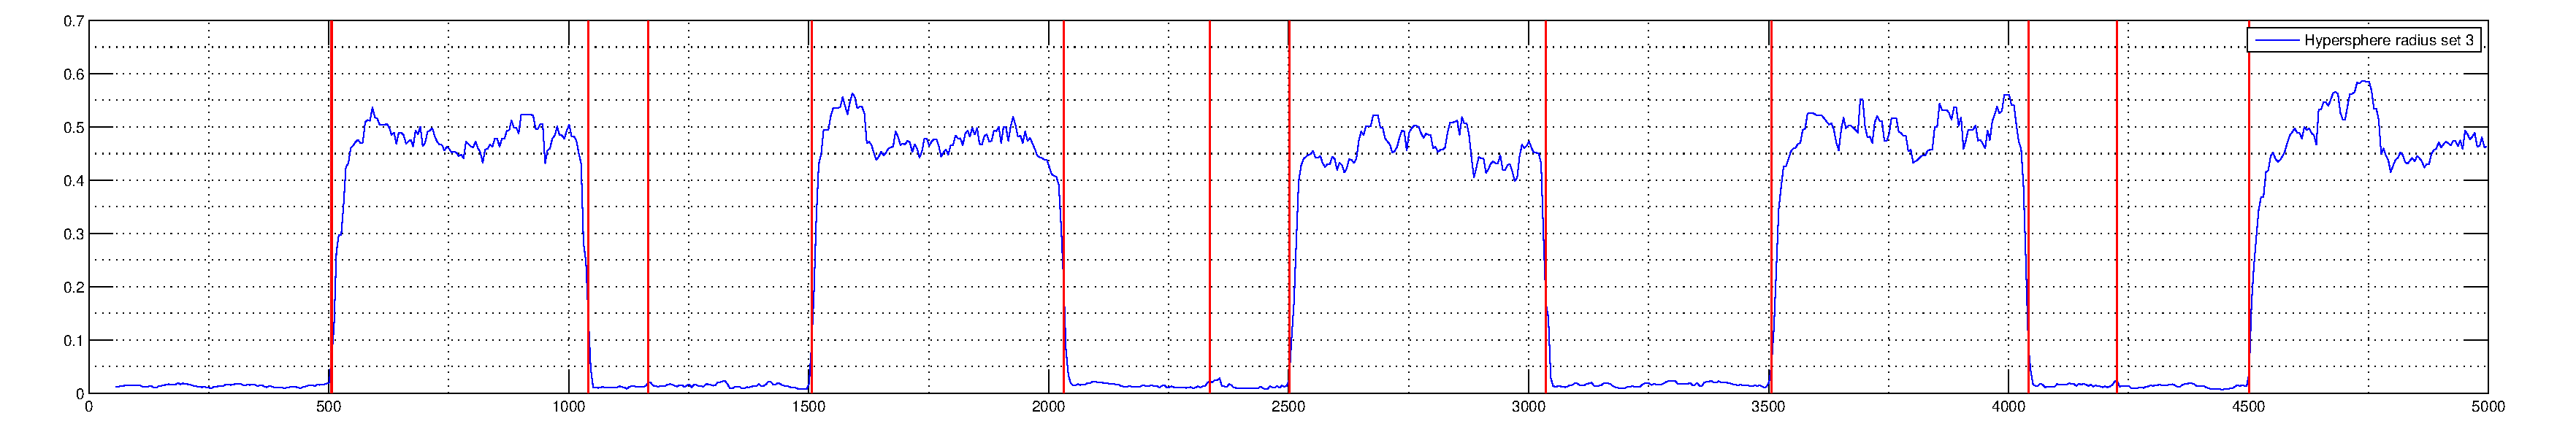
\includegraphics[width=1\textwidth]{./Figures/chapter5/set_4_results.eps}
    \caption[Alternating variance, thresholds]{\emph{Alternating variance} data set.}
    \label{fig:camci_takeuchi_alternating_variance_thresholds}
  \end{subfigure} \\

  \caption[Artificial data set results]{Hypersphere radius sizes for the four artificial data sets. The detected change points are displayed as dashed thick red vertical bars.}
  \label{fig:plots_results_artificial_data_sets}
\end{figure}